\chapter[Suporte Tecnológico]{Suporte Tecnológico}

Aqui é listado todos os programas, tecnologias, ferramentas e aparelhos que serão  usados para a produção do \textit{framework} e do robô onde será testado. 

\section{Linguagem de programação}

A linguagem em que o \textit{framework} será implementado será Java. Isso exige que o robô aonde o \textit{framework} será rodado tenha uma máquina virtual Java instalado nela. A escolha da linguagem se deu ao kit disponível para o trabalho rodar esta linguagem.

\section{Ferramentas e plugins}

Como inspiração para o tema e base para o funcionamento dos algoritmos foi analisado o software MRIT (Mobile Robotics Interactive Tool) \cite{MRIT_SITE} desenvolvido por \cite{Guzman2008}. Este software permite a simulação de algoritmos locais e globais, definindo a trajetória em meio aos obstáculos e considerando as características físicas do robô. Ele foi usado para estudo do tema e do comportamento dos algoritmos globais e será aproveitado para comparações com os resultados feitos pelo \textit{framework} e exemplificar visualmente o funcionamento dos algoritmos utilizados.

Para o desenvolvimento do projeto será usado a IDE Eclipse Indigo \cite{ECLIPSE_SITE}. O código, compilação e execução será toda feita através desta IDE, que contará com um \textit{plugin} do kit utilizado (Lejos NXT) para rodar as bibliotecas do kit e permitir a compilação devida e \textit{upload} do código para o robô. O \textit{plugin} pode ser encontrado em \cite{PLUGIN_NXT_SITE}.

Para os testes e controle de qualidade do sistema será usado o \textit{plugin} JUnit \cite{JUNIT_SITE} para testes unitários. Assim como o outro, este \textit{plugin} estará embutido à IDE. Outro plugin será o Eclemma para cobertura de código \cite{ECLEMMA_SITE}, também embutido na IDE.

\section{Lego NXT}

O kit utilizado para testar o \textit{framework} será o kit educacional da LEGO em sua segunda versão: o LEGO NXT. O robô será montado com peças de lego e movido com os motores do kit. O LEGO NXT possui um processador Atmel ARM 32 bits com \textit{clock} de 48MHz, HD de 256KB de memória \textit{flash}, memória RAM de 64KB e sistema operacional proprietário.

O kit permite a instalação de um Java adaptado para sua plataforma, o Lejos NXJ \cite{LEJOS_SITE}. O Lejos não vem instalado por padrão no kit. Para inseri-lo primeiro deve instalá-lo no computador onde será programado e então executar sua instalação via cabo USB no robô.

\begin{figure}[h]
	\centering
	\label{fig17}
		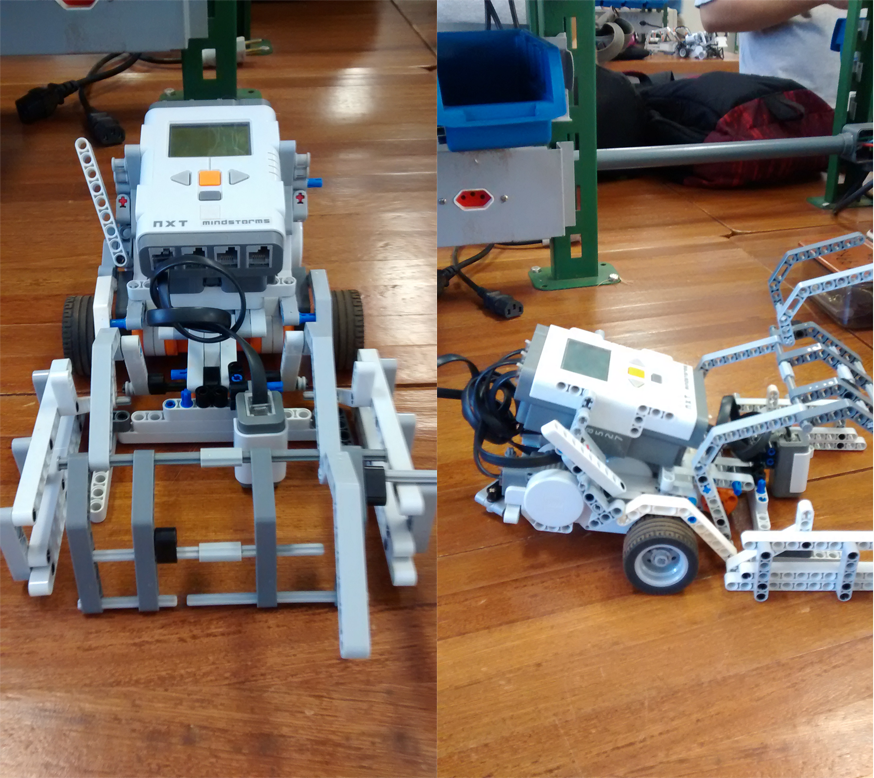
\includegraphics[keepaspectratio=true,scale=0.2]{figuras/5nxtBrick.png}
	\caption{foto do robô utilizado}
\end{figure}

\section{Differential Steering}

A estrutura física da plataforma será um \textit{differential steering} montado com os dois motores e as peças do kit já referido. O modelo terá duas rodas fixas na frente, cada uma ligada a um motor e a iguais distâncias do centro do robô. Atrás uma roda castor mantêm o equilíbrio e permanece livre para girar conforme a estrutura se locomover.

Por ter motores separados nas rodas o movimento do robô se torna mais flexível e variado, podendo girar em torno de cada roda ou do próprio eixo. Cada roda pode girar em uma velocidade diferente ou até para lados diferentes ou pode girar uma roda e manter a outra parada. Por essa liberdade e simplicidade este modelo é muito usado em robótica (\cite{Mataric2007}).

Há variações deste estilo, onde toda as rodas de um lado estão ligadas a um mesmo motor como mostra a figura a seguir.

\begin{figure}[h]
	\centering
	\label{fig18}
		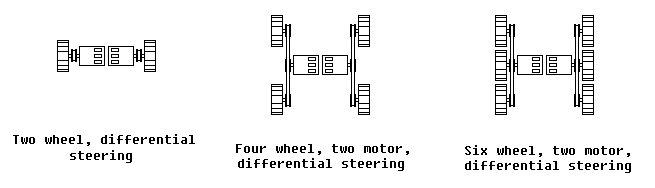
\includegraphics[keepaspectratio=true,scale=0.7]{figuras/3differentialSteering.png}
	\caption{exemplos de estruturas differential steering \cite{IMG_DIFFERENTIAL_STEERING_SITE}}
\end{figure}
